\chapter{Wasserstoffatom\label{chapter:wasserstoff}}
\lhead{Wasserstoffatom}
\rhead{}
Der bisher entwickelte Formalismus erlaubt bereits, das Wasserstoff-Atom
\index{Wasserstoff}
zu verstehen. Die Quantenmechanik erkl"art die Stabilit"at der
Materie, und sagt das Wasserstoff-Spektrum korrekt voraus.
\section{Schr"odinger-Gleichung f"ur das Wasserstoffatom}
\rhead{Schr"odingergleichung f"ur das Wasserstoffatom}
Die Hamilton-Funktion eines Elektrons im Potential eines einzelnen
Protons, welches sich im Nullpunkt des Koordinatensystems befindet,
ist
\begin{equation}
H=\frac1{2m_e}p^2 + V(r)
=\frac1{2m_e}p^2 - \frac1{4\pi\varepsilon_0}\frac{e^2}{r}.
\label{skript:h2hamilton}
\end{equation}
Darin ist $m_e$ die Masse des Elektrons, $e$ ist die Elementarladung.
$r$ ist die Entfernung eines Punktes vom Nullpunkt.
Der Impuls $p$ ist als Vektor zu verstehen, also $p^2=p_x^2+p_y^2+p_z^2$.

Wir suchen eine L"osung des quantisierten Systems mit Zustandsvektoren, die von
den Ortskoordinaten abh"angen.
Nach den Quantisierungsregeln m"ussen die Impulse in der Hamiltonfunktion
durch Ableitungsoperatoren
\begin{equation}
p_x\rightarrow \frac{\hbar}{i}\frac{\partial}{\partial x},
\qquad
p_y\rightarrow \frac{\hbar}{i}\frac{\partial}{\partial y},
\quad
\text{und}
\quad
p_z\rightarrow \frac{\hbar}{i}\frac{\partial}{\partial z}.
\label{skript:h2quant}
\end{equation}
ersetzt werden. Wendet man die Ersetzungen (\ref{skript:h2quant}) auf die
Hamilton-Funktion (\ref{skript:h2hamilton}) an, erh"alt man den Hamilton-Operator
f"ur das Wasserstoff-Atom:
\[
\hat H=-\frac{\hbar^2}{2m_e}\biggl(
\frac{\partial^2}{\partial x^2}+
\frac{\partial^2}{\partial y^2}+
\frac{\partial^2}{\partial z^2}
\biggr)-\frac1{4\pi\varepsilon_0}\frac{e^2}{r}
=-\frac{\hbar^2}{2m_e}\Delta -\frac1{4\pi\varepsilon_0}\frac{e^2}{r}.
\]
Wir suchen zeitunabh"angige Zust"ande, also Eigenfunktionen dieses
Operators. Wir erwarten eine Menge von Zustandsvektoren $|\psi\rangle$
mit zugeh"origen Eigenwerten $E$, so dass
\begin{equation}
\hat H\,|\psi\rangle = E\,|\psi\rangle.
\label{skript:h2schroedinger}
\end{equation}
(\ref{skript:h2schroedinger}) ist eine partielle Differentialgleichung.
Wir beabsichtigen nicht, eine allgemeine Theorie der partiellen
Differentialgleichungen zu entwickeln.
F"ur unsere Zwecke reicht es, eine ad hoc L"osung zu finden.

\section{Kugelkoordinaten}
\rhead{Kugelkoordinaten}
Das Eigenwertproblem (\ref{skript:h2schroedinger}) kann in kartesischen
Koordinaten nicht direkt gel"ost werden.
Dies liegt daran, dass die kartesischen
Koordinaten die vorhandene Kugelsymmetrie des Problems nicht ausreichend
ber"ucksichtigen. Es ist viel besser, Kugelkoordinaten zu verwenden.

Die Umrechnungn zwischen Kugelkoordinaten $(r,\vartheta,\varphi)$ und
kartesischen Koordinaten $(x,y,z)$ ist gegeben durch
\begin{align*}
x&=r
\sin\vartheta
\cos\varphi,
\\
y&=r
\sin\vartheta
\sin\varphi,
\\
z&=r\cos \vartheta.
\end{align*}
Eine etwas m"uhsame, im Anhang (Kapitel~\ref{chapter:kugelkoordinaten})
durchgef"uhrte Rechnung erlaubt, den Laplace-Operator in Kugelkoordinaten
auszudr"ucken:
\[
\Delta
=
\frac1{r^2}\frac{\partial}{\partial r}\biggl(
r^2\frac{\partial}{\partial r}
\biggr)
+\frac1{r^2\sin\vartheta}\frac{\partial}{\partial \vartheta}\biggl(
 \sin\vartheta \frac{\partial}{\partial\vartheta}
\biggr)
+
\frac1{r^2\sin^2\vartheta}\frac{\partial^2}{\partial\varphi^2}.
\]

\section{L"osung der Schr"odingergleichung\label{section:schroedinger}}
\rhead{L"osung der Schr"odingergleichung}
Wir suchen jetzt also L"osungen des Eigenwertproblems
(\ref{skript:h2schroedinger})
als $L^2$-Funktionen in Kugel-Koordinaten $(r,\varphi,\vartheta)$. Wir
verwenden dazu die Methode der Separation der Variablen.

\subsection{Separationsansatz}
\index{Separationsansatz}
Wir nehmen an,
dass sich die L"osung $\psi(r,\vartheta,\varphi)$ schreiben l"asst als
ein Produkt von drei Funktionen, die je nur von einer Koordinate
abh"angen. Wir setzen also an
\begin{equation}
\psi(r,\vartheta,\varphi)=R(r)\cdot
\Theta(\vartheta)\cdot
\Phi(\varphi)
\label{skript:sepansatz}
\end{equation}
und setzen dies in das Eigenwertproblem ein. Dazu brauchen wir die Ableitung
nach $r$, $\varphi$ und $\vartheta$ von $\psi(r,\varphi,\vartheta)$, doch
diese Ableitungen wirken jeweils nur auf einen der Faktoren:
\[
\frac{\partial}{\partial r}\psi(r,\vartheta,\varphi)
=
\frac{d R(r)}{d r}
\cdot \Theta(\vartheta)
\cdot  \Phi(\varphi)
+
R(r)
\cdot \Theta(\vartheta)
\cdot \underbrace{\frac{d\Phi(\varphi)}{dr}}_{=0}
+
R(r)
\cdot \underbrace{\frac{d \Theta(\vartheta)}{d r}}_{=0}
\cdot \Phi(\varphi)
=
R'(r)
\cdot \Theta(\vartheta)
\cdot \Phi(\varphi)
\]
und analog f"ur die anderen Variablen.
Wir k"onnen also so tun, als ob die Ableitungen jeweils nur auf genau
einen der Faktoren wirken.
\begin{equation}
\Delta \psi
=
\frac1{r^2}\frac{d}{dr}\bigl(r^2R'(r)\bigr)
\cdot \Theta(\vartheta)
\cdot \Phi(\varphi)
+
R(r)
\cdot \frac{1}{r^2\sin\vartheta}
\frac{d}{d\vartheta}(\sin\vartheta \Theta'(\vartheta))
\cdot \Phi(\varphi)
+
\frac{R(r)}{r^2\sin^2\vartheta}
\cdot \Theta(\vartheta)
\cdot \Phi''(\varphi)
\label{skript:separated}
\end{equation}
Man beachte, dass in allen Termen immer nur einer der Faktoren des
Separationsansatzes abgeleitet wurde.

Das Eigenwertproblem, welches zu l"osen ist, wird jetzt in Kugelkoordinaten
zu
\[
-\frac{\hbar^2}{2m_e} \Delta\psi(r,\vartheta,\varphi)
-\frac{1}{4\pi\varepsilon_0}\frac{e^2}{r}\psi(r,\vartheta,\varphi)
=E\psi(r,\vartheta,\varphi).
\]

\subsection{Separation von $\varphi$}
Keine der drei Faktoren des Ansatzes (\ref{skript:sepansatz}) f"ur
$\psi(r,\vartheta,\varphi)$ kann verschwinden, sonst erhielten wir die 
Nullfunktion, also nicht einen Eigenvektor von $\hat H$.
Nat"urlich k"onnen die Faktoren einzelne Nullstellen haben, aber ausserhalb
dieser Nullstellen kann man die Gleichung (\ref{skript:separated}) durch 
$\psi(r,\vartheta,\varphi)$ teilen. Wir erhalten
\begin{equation*}
-\frac{\hbar^2}{2m_e}\biggl(
\frac{1}{R(r)}
\frac{1}{r^2}
\frac{d}{dr}(r^2R'(r))
+
\frac{1}{\Theta(\vartheta) r^2\sin\vartheta}\frac{d}{d\vartheta}(\sin\vartheta \Theta'(\vartheta))
+
\frac{1}{r^2\sin^2\vartheta}\frac{\Phi''(\varphi)}{\Phi(\varphi)}
\biggr)
-\frac1{4\pi\varepsilon_0}\frac{e^2}{r}
=
E.
\end{equation*}
Bringen wir ausserdem alle Terme mit $\varphi$ auf die rechte Seite,
und multiplizieren mit $r^2\sin^2\vartheta$
ergibt sich
\begin{equation*}
-\frac{\hbar^2}{2m_e}
\frac{1}{R(r)}\sin^2\vartheta \frac{d}{dr}(r^2R'(r))
-
\frac{\hbar^2}{2m_e}
\frac{\sin\vartheta}{\Theta(\vartheta) }\frac{d}{d\vartheta}(\sin\vartheta \Theta'(\vartheta))
-\biggl(\frac1{4\pi\varepsilon_0}\frac{e^2}{r}
+
E\biggr)r^2\sin^2\vartheta
=
\frac{\hbar^2}{2m_e}\frac{\Phi''(\varphi)}{\Phi(\varphi)}.
\end{equation*}
Indem wir durch den Faktor $-\hbar^2/2m_e$ dividieren, wir die Gleichung
etwas "ubersichtlicher:
\begin{equation}
\frac{1}{R(r)}\sin^2\vartheta \frac{d}{dr}(r^2R'(r))
+
\frac{\sin\vartheta}{\Theta(\vartheta) }\frac{d}{d\vartheta}(\sin\vartheta \Theta'(\vartheta))
+\biggl(\frac{m_e}{2\pi\varepsilon_0\hbar^2}\frac{e^2}{r}
+
\frac{2m_eE}{\hbar^2}\biggr)r^2\sin^2\vartheta
=
-\frac{\Phi''(\varphi)}{\Phi(\varphi)}.
\label{skript:phisepariert}
\end{equation}
Die linke Seite dieser Gleichung h"angt nicht von $\varphi$ ab, also
darf auch die rechte Seite nicht von $\varphi$ abh"angen, sie muss
eine Konstante sein. Wir nennen die Konstante $m^2$ (dies wird sich
als zweckm"as\-sig herausstellen). Wir haben also aus der urspr"unglichen
partiellen Differentialgleichung eine gew"ohnliche Differentialgleichung
\[
-\frac{\Phi''(\varphi)}{\Phi(\varphi)}=m^2
\quad\Leftrightarrow\quad
\Phi''(\varphi)=-m^2\Phi(\varphi)
\]
f"ur die Funktion $\Phi(\varphi)$ gefunden.
Die L"osungen einer solchen Differentialgleichung zweiter Ordnung sind
wohl bekannt: $e^{im\varphi}$ und $e^{-im\varphi}$. Damit die Funktion
periodisch wird, muss $m$ eine nat"urliche Zahl sein, $m=0,1,2,\dots$.

\subsection{Separation von $r$ und $\vartheta$}
In der Gleichung (\ref{skript:phisepariert}) kommt auf der linken Seite nur
noch $r$ und $\vartheta$ vor.  Die rechte Seite haben wir inzwischen auf
die m"oglichen Werte $m^2$ reduziert. Teilen wir die Gleichung durch
$\sin^2\vartheta$, und bringen die von $\vartheta$ abh"angenden Terme
auf die rechte Seite, erhalten wir die Gleichung
\begin{equation}
-\frac{\hbar^2}{2m_e}
\frac{1}{R(r)}\frac{d}{dr}\bigl(r^2R'(r)\bigr)
-\biggl(\frac{1}{4\pi\varepsilon_0}\frac{e^2}{r}
+
E
\biggr)r^2
=
\frac{\hbar^2}{2m_e}
\biggl(
\frac1{\sin\vartheta\Theta(\vartheta) }
\frac{d}{d\vartheta}\bigl(\sin\vartheta \Theta'(\vartheta)\bigr)
-
\frac{m^2}{\sin^2\vartheta}
\biggr).
\label{skript:thetasepariert}
\end{equation}
Die linke Seite von (\ref{skript:thetasepariert}) h"angt nicht von $\vartheta$
ab, also kann auch die rechte Seite nicht von $\vartheta$ abh"angen.
Ebenso h"angt die rechte Seite nicht von $r$, also kann auch die linke
nicht von $r$ abh"angen. Beide Seiten m"ussen also konstant sein,
wir nennen die Konstante $\lambda$.

\subsection{Abh"angigkeit von $\vartheta$}
Die Funktion $\Theta(\vartheta)$ auf der rechten Seite ist eigentlich
eine Funktion von $z=\cos\vartheta$. Wir schreiben
$Z(z)=Z(\cos\vartheta)=\Theta(\vartheta)$. Die Ableitung nach $\vartheta$
kann dann umgeschrieben werden in eine Ableitung nach $z$
\begin{align*}
\Theta'(\vartheta)&=
\frac{d}{d\vartheta}Z(z)=Z'(z)\frac{dz}{d\vartheta}=-\sin\vartheta Z'(z),
\\
\frac{d}{dz}
&=
-\frac1{\sin\vartheta}\frac{d}{d\vartheta}.
\end{align*}
Nat"urlich gilt auch $1-z^2=\sin^2\vartheta$, so dass die rechte Seite
von (\ref{skript:thetasepariert}) zu
\begin{equation}
-
\frac1{\Theta(\vartheta)}
\frac1{\sin\vartheta}
\frac{d}{d\vartheta}\biggl(
\sin^2\vartheta \frac1{\sin\vartheta}\frac{d}{d\vartheta}\Theta'(\vartheta)
\biggr)
+
\frac{m^2}{\sin^2\vartheta}
=
-\frac1{Z(z)}\frac{d}{dz}\biggl(
(1-z^2)\frac{d}{dz}Z(z)
\biggr)
+
\frac{m^2}{1-z^2}
\end{equation}
wird. Dieser Ausdruck muss konstant sein, wir nennen die Konstante 
$\lambda$:
\begin{equation}
-\frac1{Z(z)}\frac{d}{dz}\biggl(
(1-z^2)\frac{d}{dz}Z(z)
\biggr)
+
\frac{m^2}{1-z^2}
=\lambda
\end{equation}
oder
\begin{equation}
\frac{d}{dz}\biggl(
(1-z^2)\frac{d}{dz}Z(z)
\biggr)
+\biggl(\lambda
-
\frac{m^2}{1-z^2}
\biggr)Z(z)
=0.
\label{skript:legendregleichung}
\end{equation}

\subsubsection{Spezialfall $m=0$}
Wir untersuchen diese L"osung zun"achst f"ur den Spezialfall $m=0$,
d.~h.~wir m"ussen die Differentialgleichung
\begin{equation}
\frac{d}{dz}\biggl(
(1-z^2)\frac{d}{dz}Z(z)
\biggr)
+\lambda Z(z)=0
\label{skript:Zequation}
\end{equation}
l"osen.
Dies ist die sogenannte Legendresche Differentialgleichung,
\index{Legendre-Differentialgleichung}
deren L"osung in einer guten Formelsammlung gefunden werden k"onnen.

Wir versuchen eine L"osung in Form eines Polynoms vom
Grade $l$ zu finden, also 
\begin{equation}
P_l(z)=a_0+a_1z+\dots+a_lz^l.
\label{skript:legendreansatz}
\end{equation}
Setzen wir dies in die Gleichung~(\ref{skript:Zequation}) ein, und betrachten nur die
Terme vom Grad $z^l$:
\begin{align*}
\frac{d}{dz}(-z^2la_lz^{l-1})
+
\lambda a_lz^l&=0
\\
-l(l+1)a_lz^l+\lambda a_lz^l&=0,
\end{align*}
Es folgt, dass $\lambda = l(l+1)$ sein muss, wobei $l$ eine ganze
Zahl sein muss.

Wie jede Differentialgleichung zweiter Ordnung hat die Legendresche
Differentialgleichung ausser den $P_l$ auch noch eine L"osung
$Q_l$, diese ist jedoch nicht beschr"ankt und kommt daher als L"osungsfunktion
f"ur unser Problem nicht in Frage.

\subsubsection{Legendre-Polynome}
\index{Legendre-Polynom}
Indem man den Ansatz (\ref{skript:legendreansatz}) f"ur alle Koeffizienten
auswertet, nicht nur f"ur $a_l$, kann man die Polynome $P_l(z)$ 
bestimmen, sie heissen Legendre-Polynome.
"Uber die Jahre wurde eine umfangreiche Theorie der Legendre-Polynome
aufgebaut, so gilt zum Beispiel die folgende Formel von Rodrigues
\[
P_l(z)=\frac1{2^ll!}\frac{d^l}{dz^l}(z^2 - 1)^l.
\]
Die Legendre-Polynome sind orthogonal.

%Durch Einsetzen in die Differentialgleichung kann man verifizieren,
%dass dies tats"achlich eine L"osung ist:
%\begin{align*}
%\frac{d}{dz}\biggl(
%(1-z^2)\frac{d}{dz}
%\frac1{2^ll!}\frac{d^l}{dz^l}(z^2 - 1)^l.
%\biggr)
%&=
%\frac1{2^ll!}
%\frac{d}{dz}\biggl(
%(1-z^2)
%\frac{d^l}{dz^l}l(z^2 - 1)^{l-1}2z.
%\biggr)
%\\
%&=
%\frac1{2^ll!}
%\biggl(
%(-2z)
%\frac{d^l}{dz^l}l(z^2 - 1)^{l-1}2z.
%+
%(1-z^2)
%\frac{d^l}{dz^l}l\frac{d}{dz}\bigl((z^2 - 1)^{l-1}2z\bigr)
%\biggr)
%\\
%\end{align*}

\subsubsection{Der Fall $m\ne 0$}
F"ur den allgemeinen Fall mit beliebigem $m$ m"ussen L"osungen der
Gleichung
\begin{equation}
\frac{d}{dz}\biggl((1-z^2)\frac{d}{dz}Z(z)\biggr)
+\biggl(\lambda -\frac{m^2}{1-z^2}\biggr)Z(z)=0
\end{equation}
gefunden werden. Man kann zeigen, dass die Funktionen
\[
P_l^m(z)=
(1-z^2)^{\frac{m}2}\frac{d^m}{dz^m}P_l(z),
\qquad
0\le m\le l
\]
L"osungen f"ur $\lambda=l(l+1)$ sind.
Auch diese allgemeineren Funktionen $P_l^m(z)$ sind orthogonal.

\subsection{Abh"angigkeit von $r$}
Die Funktion $R(r)$ erf"ullt die Differentialgleichung
\begin{align}
-\frac{\hbar^2}{2m_e} \frac{1}{r^2}\frac{d}{dr}\bigl(r^2R'(r)\bigr)
-
\biggl(\frac{e^2}{4\pi\varepsilon_0r} + E \biggr) R(r)
&=
\frac{\hbar^2}{2m_e}\frac{\lambda}{r^2}
R(r).
\label{skript:radialgleichung}
\end{align}
\begin{figure}
\centering
\includegraphics{graphics/h-1.pdf}
\caption{Durch den Drehimpuls modifiziertes effektives Potential.
\label{skript:modifiziertes-potential}}
\end{figure}%
\index{Potential!effektives}%
Wir wissen bereits, dass $\lambda=l(l+1)$.
Ausserdem k"onnen wir die ganze Gleichung durch $\hbar^2/2m_e$ teilen
und die Ableitung nach $r$ auf der linken Seite ausrechnen. 
Wir erhalten dann die Gleichung
\begin{align}
R''(r)+\frac{2}{r}R'(r)
+\frac{2m_e}{\hbar^2}
\biggl(\frac{e^2}{4\pi\varepsilon_0r} + E \biggr) R(r)
-\frac{l(l+1)}{r^2}
R(r)
&=0.
\label{skript:radialgleichung2}
\end{align}
In den folgenden Abschnitten suchen wir L"osungen dieser Gleichung.
Es wird sich zeigen, dass nur f"ur eine diskrete Menge von $E$-Werten
"uberhaupt eine L"osung existiert.

\subsubsection{Modifiziertes Potential}
Schreiben wir
\begin{equation}
A=\frac{2m_eE}{\hbar^2}
\qquad\text{und}\qquad
B=\frac{m_ee^2}{4\pi\varepsilon_0\hbar^2},
\label{skript:AundB}
\end{equation}
k"onnen wir die Gleichung (\ref{skript:radialgleichung2})
noch etwas "ubersichtlicher als
\begin{equation}
R''(r)+\frac2{r}R'(r)+\biggl(A+\frac{2B}r-\frac{l(l+1)}{r^2}\biggr)R(r)=0
\label{skript:hreduziert}
\end{equation}
schreiben.
In dieser Form erkennt man, dass $l\ne 0$
das Potential modifiziert mit einem Term
$\sim\frac1{r^2}$ (Abbildung~\ref{skript:modifiziertes-potential}).
Er bewirkt, dass sich das Elektron bevorzugt in einer
gewissen Entfernung vom Kern aufh"alt, die umso gr"osser ist, je
gr"osser $l$ ist.
Wir werden im n"achsten Kapitel lernen, dass $l$ die Bedeutung des
Drehimpulses hat.

Wir erwarten, dass das Elektron mit gr"osster Wahrscheinlichkeit
in der N"ahe des Minimums des effektiven Potentials zu finden ist.
Wir k"onnen daher aus der Form des effektiven Potentials bereits
schliessen, dass sich die Elektronen bevorzugt auf Schalen befinden
werden, deren Radius durch den Drehimpuls $l(l+1)$ gegeben ist.

\subsubsection{Verhalten f"ur $r\to\infty$}
Wir interessieren uns f"ur an das Atom gebundene Elektronen, also
Zust"ande mit negativer Energie.
In diesem Fall ist wegen (\ref{skript:AundB}) auch $A$ negativ.
Aus den Beispielen des Kapitels~\ref{chapter:quantisierung} wissen wir,
dass in diesem Fall f"ur grosse Entfernung die Wellenfunktion exponentiell
abfallen muss.
Wir untersuchen daher das Verhalten der Gleichung (\ref{skript:hreduziert})
f"ur grosse $r$.
Indem wir die Terme mit $1/r$ und $1/r^2$ vernachl"assigen, da sie 
f"ur grosses $r$ klein sind, erhalten wir f"ur grosse $r$ die Differentialgleichung
\[
R''(r)+AR(r)=0,
\]
die die L"osungen
\[
R(r)=K_\pm e^{\pm\sqrt{-A}r}
\]
hat.
Die L"osung mit dem positiven Vorzeichen kommt nicht in Frage, weil
sie f"ur grosse $r$ exponentiell anw"achst.

\subsubsection{``Separation'' des asymptotischen Verhaltens}
Die Funktion $Ke^{-\sqrt{-A}r}$ ist zwar eine asymptotische L"osung
f"ur grosse $r$, f"ur kleine $r$ muss sie aber nochmals modifiziert
werden.
Wir versuchen daher f"ur die Funktion $R(r)$ einen Ansatz der Form
\begin{equation}
R(r)=w(r)e^{-\sqrt{-A}r}.
\label{skript:Ransatz}
\end{equation}
Dies entspricht dem Separationsansatz f"ur die Funktion
$\psi(r,\vartheta,\varphi)$, nur dass hier in einer Funktion nur einer
Variablen das asymptotische Verhalten, ausgedr"uckt durch den
Exponentialfaktor, vom lokalen Verhalten, ausgedr"uckt durch $w(r)$,
getrennt wird.

Wir brauchen davon die erste und zweite Ableitung
\begin{align*}
R'(r)&=(w'(r)-\sqrt{-A}w(r))e^{-\sqrt{-A}r},
\\
R''(r)&=(w''(r)-2\sqrt{-A}w'(r)-Aw(r))e^{-\sqrt{-A}r},
\end{align*}
um sie in die Differentialgleichung~(\ref{skript:hreduziert}) einzusetzen.
Nach Division durch den immer positiven Exponentialfaktor
erhalten wir die Differentialgleichung
\begin{align}
&&
w''(r)-2\sqrt{-A}w'(r)-Aw(r)
+\frac2{r}(w'(r)-\sqrt{-A}w(r))
+\biggl(A+\frac{2B}r-\frac{l(l+1)}{r^2}\biggr)w(r)&=0
\notag
\\
&\Leftrightarrow&
w''(r)+\biggl(\frac{2}{r}-2\sqrt{-A}\biggr)w'(r)
+\biggl(\frac{2B-2\sqrt{-A}}{r}-\frac{l(l+1)}{r^2}\biggr)w(r)&=0
\notag
\\
&\Leftrightarrow&
\underbrace{
w''(r)+\frac{2}{r}w'(r)
}_{\text{\normalsize\ding{192}}}
\underbrace{\mathstrut-2\sqrt{-A}w'(r)
+\frac{2B-2\sqrt{-A}}{r} w(r)
}_{\text{\normalsize\ding{193}}}
\underbrace{\mathstrut-\frac{l(l+1)}{r^2}w(r)}_{\text{\normalsize\ding{194}}}&=0
\label{skript:wequation}
\end{align}
f"ur $w(r)$.

\subsubsection{Polynomansatz f"ur $w(r)$}
Wir erwarten, dass das wesentliche Verhalten der Funktion $R(r)$ 
f"ur $r\to\infty$ bereits durch den Exponentialfaktor abgehandelt ist.
Die Funktion $w(r)$ muss also nur noch das Verhalten f"ur kleine $r$
abbilden.
Sie darf daher im Vergleich zu der Exponentialfunktion nur langsam wachsen,
ein Polynom w"urde diese Bedingung erf"ullen.
Wir schreiben daher
\[
w(r)=\sum_{k=0}^N a_kr^k,
\]
und versuchen zu ermitteln, f"ur welche Werte von $A$ und $B$ diese
Wahl von $w(r)$ "uberhaupt m"oglich ist.

Auch in diesem Fall brauchen wir die ersten und zweiten Ableitungen von
$w(r)$
\[
\begin{aligned}
w'(r)&=\sum_{k=1}^Nka_kr^{k-1}
&&\text{und}
&
w''(r)&=\sum_{k=2}^Nk(k-1)a_kr^{k-2},
\end{aligned}
\]
um sie in die Gleichung (\ref{skript:wequation}) einsetzen zu k"onnen.

\subsubsection{Koeffizientenvergleich}
Nach dem Einsetzen unseres Ansatzes f"ur $w(r)$ in die Gleichung
(\ref{skript:wequation})
m"ussen alle Koeffizienten der Potenzen von $r$ verschwinden.
Man beachte, dass die Ableitung wie auch die Division durch $r^2$ den
Grad der Potenzen von $r$ reduziert.
Wir beginnen also damit, einzelne Terme der Gleichung
(\ref{skript:wequation}) zusammenzufassen und sie so zu schreiben,
dass wir immer Summen erhalten, in denen $k$ von $1$ bis $N$ l"auft, 
und in denen immer die Potenz $r^{k-2}$ vorkommt.
Damit wird es besonders einfach werden, den Koeffizientenvergleich
durchzuf"uhren.

Nat"urlich k"onnen dabei Terme stehen bleiben, die
sich nicht in dieser Form schreiben lassen.
Dies wird uns sp"ater zus"atzliche Bedingungen f"ur die Koeffizienten $a_k$
geben.

Zun"achst betrachten wir den Teil
\begin{align*}
\text{\ding{192}}=
w''(r)+\frac2{r}w'(r)
&=
\sum_{k=2}^N k(k-1)a_kr^{k-2} + \frac{2}{r}\sum_{k=1}^Nka_kr^{k-1}
\\
&=
\sum_{k=2}^N\bigl(k(k-1)a_kr^{k-2} + 2ka_kr^{k-2}\bigr) + \frac{2a_1}{r}
\\
&=
\sum_{k=2}^Nk(k+1)a_kr^{k-2} + \frac{2a_1}r
\\
&=
\sum_{k=1}^Nk(k+1)a_kr^{k-2}.
\end{align*}
Analog k"onnen wir die Terme 
\begin{align*}
\text{\ding{193}}&=
\frac{2B-2\sqrt{-A}}{r}w(r)-2\sqrt{-A}w'(r)
\\
&=
(2B-2\sqrt{-A})\frac{a_0}{r}
+
(2B-2\sqrt{-A})\sum_{k=1}^Na_kr^{k-1}
-2\sqrt{-A}\sum_{k=1}^Nka_kr^{k-1}
\\
&=
(2B-2\sqrt{-A})\frac{a_0}{r}
+
\sum_{k=1}^N
(2B-2\sqrt{-A}
-2k\sqrt{-A})a_kr^{k-1}
\\
&=
(2B-2\sqrt{-A})\frac{a_0}{r}
+
\sum_{k=1}^N
(2B-2(k+1)\sqrt{-A})a_kr^{k-1}
\\
&=
(2B-2\sqrt{-A})\frac{a_0}{r}
+
\sum_{k=2}^{N+1}
(2B-2k\sqrt{-A})a_{k-1}r^{k-2}
\\
&=
\sum_{k=1}^{N+1}
(2B-2k\sqrt{-A})a_{k-1}r^{k-2}
\end{align*}
behandeln.
Auch den Drehimpulsterm k"onnen wir in dieser Form schreiben:
\begin{align*}
\text{\ding{194}}=
-\frac{l(l+1)}{r^2}w(r)
&=
-l(l+1)\frac{a_0}{r^2}
-
\sum_{k=1}^Nl(l+1)a_kr^{k-2}.
\end{align*}
Damit haben wir alle Teile in der vorgeschlagenen Form als Summen
"uber $k$ von $1$ bis $N$ geschrieben mit Potenzen $r^{k-2}$.
Ein spezieller Term $r^{-2}$ ist hinzu gekommen.

Nach diesen Vorbereitungen k"onnen wir jetzt den Koeffizientenvergleich
durchf"uhren, indem wir alle Terme zusammennehmen:
\begin{equation}
\text{\ding{192}}
+
\text{\ding{193}}
+
\text{\ding{194}}
=
\sum_{k=1}^{N}
\biggl(
\bigl(
\underbrace{
k(k+1)
}_{\text{\normalsize\ding{192}}}
-\underbrace{
l(l+1)
}_{\text{\normalsize\ding{194}}}
\bigr)a_k
+
\underbrace{
2(B-k\sqrt{-A})a_{k-1}
}_{\text{\normalsize\ding{193}}}
\biggr)r^{k-2}
\underbrace{
\mathstrut
-l(l+1)\frac{a_0}{r^2}.
}_{\text{\normalsize\ding{194}}}
\label{skript:wkoeffizientenvergleich}
\end{equation}
Zun"achst f"allt auf, dass der Term $1/r^2$ nicht durch einen anderen
Term kompensiert werden kann, es muss also gelten
\[
a_0l(l+1)=0,
\]
der Koeffizient $a_0$ kann nur dann nicht verschwinden, wenn $l=0$ ist.

Wenn $l>0$ ist, muss $a_0$ verschwinden, aber es k"onnten auch noch
weitere Terme verschwinden.
Sei $k\ge 1$ der kleinste Index, f"ur den $a_k$ nicht verschwindet.
Nat"urlich ist dann $a_{k-1}=0$.
Der Klammerterm in der Summe von (\ref{skript:wkoeffizientenvergleich})
besteht dann nur noch aus dem ersten Summanden, der daher verschwinden
muss
\[
(k(k+1)-l(l+1))a_k=0.
\]
Wegen $a_k\ne 0$ k"onnen wir schliessen, dass $k(k+1)-l(l+1)=0$,
oder $k=l$.
Also ist der erste nicht verschwindende
Koeffizient in $w(r)$ derjenige mit dem Index $l$.

Den Klammerterm in der Summe von (\ref{skript:wkoeffizientenvergleich})
k"onnen wir jetzt nutzen, um eine Rekursionsformel f"ur $a_k$
aufzustellen
\begin{gather}
(k(k+1)-l(l+1))a_k+2(B-k\sqrt{-A})a_{k-1} =0
\notag
\\
\Rightarrow\qquad
a_k=-2\frac{B-k\sqrt{-A}}{k(k+1)-l(l+1)} a_{k-1}.
\label{skript:wrekursion}
\end{gather}
Wir erwarten, dass die $a_k$ ab einem bestimmten Index $n$ verschwinden.
Das ist nur m"oglich, wenn der Z"ahler in (\ref{skript:wrekursion})
verschwindet. Es gibt also einen Index $n$, f"ur den gilt
\begin{align*}
B-n\sqrt{-A}&=0,
\\
\frac{B}{n}&=\sqrt{-A},
\\
A&=-\frac{B^2}{n^2}.
\end{align*}
In (\ref{skript:AundB}) hatten wir $A$ durch die Energie $E$ ausgedr"uckt,
wir k"onnen also durch aufl"osen nach $E$ die Energie durch den Index $k$
ausdr"ucken:
\begin{align}
\frac{2m_eE}{\hbar^2}
&=
-
\biggl(
\frac{m_ee^2}{4\pi\varepsilon_0\hbar^2}
\biggr)^2
\frac{1}{n^2}
\notag
\\
E&=-\frac{m_e e^4}{32\pi^2\varepsilon_0^2\hbar^2}\cdot\frac{1}{n^2}
=-\frac{m_ee^4}{8\varepsilon_0^2h^2}\cdot\frac{1}{n^2}.
\label{skript:henergy}
\end{align}
Die Energie h"angt also nur von $n$ ab, nicht von $l$ oder $m$.

Die Quantenzahl $n$ ist der Index, ab dem all Koeffizienten verschwinden,
also hat das Polynom $w(r)$ den Grad $n-1$.
Andererseits ist $l$ der Index des ersten nicht verschwindenden Koeffizienten
von $w(r)$, $w(r)$ hat also mindestens den Grad $l$. Es folgt $0\le l < n$.

\section{Spektrum des Wasserstoffatoms}
\rhead{Spektrum}
\index{Spektrum}
Die L"osung der Schr"odingergleichung im vorangegangenen Abschnitt
hat gezeigt, dass der Hamiltonoperator des Wasserstoffatoms zu jeder ganzen
Zahl $l\ge 0$ eine Eigenfunktion der Form
\[
|n,l,m\rangle
=
P_l^m(\cos\vartheta) e^{im\varphi}e^{-rB/n}w_{nl}(r)
,\quad
B=\frac{m_ee^2}{4\pi\varepsilon_0\hbar^2}
\]
hat mit $n>0$, $m=-l,-l+1,\dots,l-1,l$.
Die zugeh"orige Energie ist
\[
E_n=-\frac{m_ee^4}{8\varepsilon_0^2h^2}\cdot \frac1{n^2}.
\]
Die Energie eines Zustandes h"angt nur von $n$ ab, nicht von $l$ oder $m$.
Bei einem "Ubergang zwischen zwischen Zust"anden mit Quantenzahlen $n_1$ und
$n_2$ wird ein Energiequantum der Gr"osse
\begin{equation}
\Delta E
=
-\frac{m_ee^4}{8\varepsilon_0^2h^2}
\biggl(
\frac{1}{n_1^2}
-
\frac{1}{n_2^2}
\biggr)
=
-13.606\text{eV}
\biggl(
\frac{1}{n_1^2}
-
\frac{1}{n_2^2}
\biggr)
\end{equation}
ausgestrahlt oder absorbiert.
Die Frequenz des ausgestrahlten oder absorbierten Lichtes ist h"angt
mit der Energie "uber $h\nu=\Delta E$ zusammen, und diese mit der
Wellenl"ange durch $\lambda = c/\nu$.
Damit bekommen wir f"ur die Wellenl"ange die Formel
\begin{align}
\frac{1}{\lambda}
&=
\frac{m_ee^4}{8\varepsilon_0^2h^3c}
\biggl(
\frac{1}{n_1^2}
-
\frac{1}{n_2^2}
\biggr)
=
R_{\text{H}}
\biggl(
\frac{1}{n_1^2}
-
\frac{1}{n_2^2}
\biggr)
=
1.0974\cdot 10^7\frac1{\text{m}}
\biggl(
\frac{1}{n_1^2}
-
\frac{1}{n_2^2}
\biggr).
\notag
\\
\lambda
&=
\frac{n_1^2n_2^2}{n_2^2-n_1^2}
\cdot
91.127\text{nm}.
\label{skript:wellenlaengenformel}
\end{align}
Die Konstante $R_{\text{H}}$ heisst die Rydberg-Konstante des
Wasserstoffs.
\index{Rydberg-Konstante}
Die daraus berechneten Wellenl"angen sind in der
Tabelle~\ref{skript:h2wellenlaengen} zusammengestellt, die
Zust"ande sind im Zustandsdiagramm in Abbildung~\ref{skript:zustandsdiagramm}
dargestellt, die zugeh"origen Wellenl"angen in der
Abbildung~\ref{skript:hspektrallinien}.
Die "Uberg"ange zum Grundzustand werden in der Lyman-Serie zusammengefasst.
\index{Lyman-Serie}
Diese Spektrallinien befinden sich im ultravioletten Teil des Spektrums.
"Uberg"ange von einem h"oheren Zustand zum Zustand mit $n=2$ 
heissen Balmer-Serie nach dem Basler Mathematiklehrer Johann Jakob Balmer,
der die Formel (\ref{skript:wellenlaengenformel}) f"ur die Wellenl"ange 
im Jahre 1885 gefunden hat.
\index{Balmer-Serie}
\index{Balmer!Johann Jakob}
F"ur kleine Werte von $n_2$ liegen die Balmer-Linien im sichtbaren Bereich.
Besonders wichtig ist die Balmer-Linie mit $n_2=3$, die auch H-$\alpha$
heisst.
Abbildung~\ref{skript:sonnehalpha} zeigt die Sonne im H-$\alpha$-Licht,
solche schmalbandigen Aufnahmen geben Aufschluss dar"uber, welche Art von
Prozessen wo auf der Sonnenoberfl"ache ablaufen.
F"ur die geplante Solar Orbiter-Mission der ESA soll mit dem Instrument
EUI (Extreme Ultraviolett Imager) in die Lage versetzt werden, Bilder
der Sonne in der Ly-$\alpha$-Linie aufzunehmen.
\index{Paschen-Serie}
\index{EUI}
\index{Solar Orbiter}

\begin{figure}
\centering
\includegraphics[width=\hsize]{graphics/h-3.pdf}
\caption{Spektrallinien des Wasserstoffatoms, die Linien einer Serie jeweils
in einer eigenen Farbe
\label{skript:hspektrallinien}}
\end{figure}


\begin{table}
\begin{center}
\begin{tabular}{crrrrrr}
\hline
Serie:&  Lyman  &  Balmer & Paschen          & Bracket &  Pfund  & Humphreys \\
$n_2$ & $n_1=1$ & $n_1=2$ & $n_1=3$          & $n_1=4$ & $n_1=5$ & $n_1=6$   \\
\hline
    2 &  121.57 &         &                  &         &         &           \\
    3 &  102.57 &   656.3 &                  &         &         &           \\
    4 &   97.25 &   486.1 &  1875\phantom{.0}&         &         &           \\
    5 &   94.97 &   434.0 &  1282\phantom{.0}&  4051   &         &           \\
    6 &   93.78 &   410.2 &  1094\phantom{.0}&  2625   &   7460  &           \\
    7 &   93.03 &   397.0 &  1005\phantom{.0}&  2166   &   4654  & 12370     \\
    8 &   92.57 &   388.8 &   954.6          &  1944   &   3741  &  7503     \\
    9 &   92.27 &   383.4 &   922.9          &  1817   &   3297  &  5908     \\
   10 &   92.05 &   379.7 &   901.3          &  1736   &   3039  &  5129     \\
   11 &   91.89 &   377.0 &   886.0          &  1680   &   3038  &  4673     \\
\hline
\end{tabular}
\end{center}
\caption{Wellenl"ange der Spektrallinien des Wasserstoffspektrums
\label{skript:h2wellenlaengen}}
\index{Bracket-Serie}
\index{Pfund-Serie}
\index{Humphreys-Serie}
\end{table}

\begin{figure}
\centering
\includegraphics{graphics/h-2.pdf}
\caption{Zustandsdiagramm des Wasserstoffatoms
\label{skript:zustandsdiagramm}}
\end{figure}

\begin{figure}
\centering
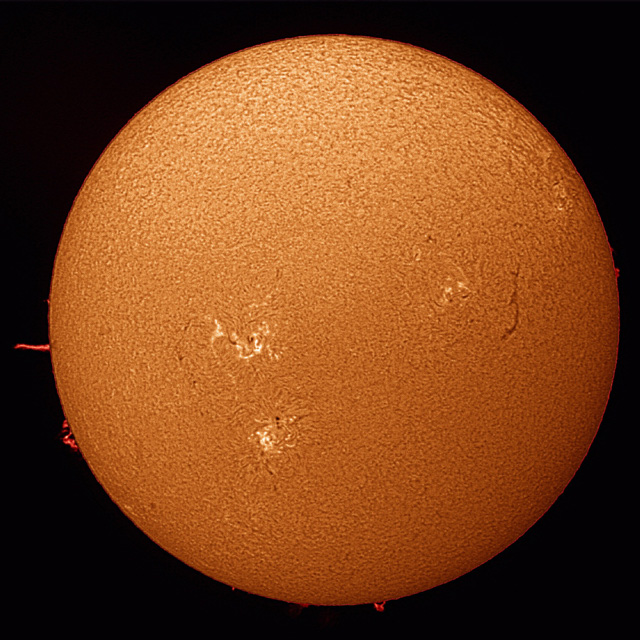
\includegraphics[width=0.6\hsize]{images/Sonne-Halpha.jpg}
\caption{Sonne im Lichte der H-$\alpha$ Spektrallinie. Im Gegensatz
zu breitbandigen Bildern, die im Wesentlichen die Intensit"at der
Scharzk"orperstrahlung und damit die Temperatur der Sonne zeigen,
geben H-$\alpha$-Bilder Auskunft "uber die Lokalisierung von Prozessen,
in denen "Uberg"ange in Wasserstoffatomen zeigen.
(Bildquelle: Wikipedia)
\label{skript:sonnehalpha}}
\end{figure}

Unsere L"osung kann auch dazu verwendet werden, das Spektrum eines
positiven Helium-Ions oder anderer stark ionisierter Atome zu berechnen.
Dazu ist die Ladung $e$ durch die effektive Ladung $Ze$ des Atomkernes
zu ersetzen, man findet die Formel
\[
\lambda = \frac{8\varepsilon_0^2h^3c}{m_eZ^2e^4}
\frac{n_1^2n_2^2}{n_2^2-n_1^2}.
\]

\section{Orbitale\label{section:orbitale}}
\rhead{Orbitale}
\index{Orbital}
Die L"osung der Schr"odinger-Gleichung in Abschnitt~\ref{section:schroedinger} 
zeigt, welche geometrische Form die Wellenfunktionen der Atome haben.
Man nennt diese Ein-Elektronen-Wellenfunktionen auch Orbitale.

Bindungen zwischen Atomen kann man sich vorstellen als Konfigurationen,
in denen Atome derart angeordnet sind, so dass die Bereiche hoher
Wahrscheinlichkeitsdichte der Orbitale der beiden Atome sich "uberlagern.
Traditionell werden die Orbitale zu verschiedenen $l$-Werten mit den
Buchstaben s, p, d, f bezeichnet.
\index{Atombindung}

Da alle Orbitale mit gleichem $n$ die gleiche Energie haben, sind auch
Linearkombinationen von solchen Orbitalen Eigenzust"ande des Atoms.
Solche Orbitale werden auch Hybridorbitale genannt, und mit
Buchstabenkombinationen wie $\text{sp}^2$ oder $\text{sp}^3$ bezeichnet.
Hybridorbitale erm"oglichen zus"atzliche Geometrien f"ur atomare Bindungen.

\subsection{s-Orbitale}
\index{s-Orbital}
Die s-Orbitale geh"oren zu $l=0$ und damit auch zu $m=0$.
Das zugeh"orige Legendre-Polynom ist eine Konstante ebenso wie die
Funktion $\Phi(\varphi)$.
Die s-Orbitale sind somit kugelsymmetrisch.

Die Radialfunktionen $w_{n0}(r)$ sind Polynome vom Grad $n-1$.
Im Grundzustand ist $w_{10}(r)$ eine Konstante.
Die Rekursionsformel f"ur die Koeffizienten von $w_{n0}(r)$ ist
\[
a_k=-2B\frac{1-\frac{k}{n}}{k(k+1)}a_{k-1}.
\]
Den Faktor $2B$ kann man eliminieren, indem man statt der Variablen $r$
die Variable $\varrho$ w"ahlt so, dass $r=2B \varrho$.
Dr"uckt man $w$ in dieser neuen Variablen aus, erh"alt man ein neues
Polynom $\tilde w_{nl}(\varrho)$, die Rekursionsformel f"ur die 
Koeffizienten $\tilde a_k$ von $\tilde w_{nl}(\varrho)$ h"angt nicht mehr
von $B$ ab:
\[
\tilde a_k = -\frac{1-\frac{k}{n}}{k(k+1)}\tilde a_{k-1}.
\]
Die Radialfunktion $R_{n0}(r)$ kann auch in der Variablen $\varrho$
geschrieben werden, sie lautet
\[
\tilde R_{n0}(\varrho)=\tilde w_{n0}(\varrho)e^{-\varrho/2n}.
\]
Mit zunehmendem $n$ steigt der Grad und damit die Anzahl der
Nullstellen von $\tilde w_{n0}$ an, es entstehen zus"atzlich lokale
Maxima, die Wahrscheinlichkeit, dass man das Elektron in gr"osserer
Entfernung vom Kern findet, steigt also an.

Das andere Extrem sind die Zust"ande mit maximalem $l=n-1$.
In diesem Fall ist $\tilde w_{nl}(\varrho)$ nur ein Monom.
Je gr"osser $n$ ist, desto schneller steigt $\tilde w_{nl}(\varrho)$ 
mit $\varrho$ an.
Der Exponentialfaktor f"allt mit gr"osser werdendem $n$ immer
langsamer ab, es ist also erst recht davon auszugehen, dass f"ur gr"osseres
$n$ sich das Elektron im Mittel weiter vom Kern entfernt aufhalten wird
(Abbildung~\ref{skript:radialgraphs-maxl}).

\begin{figure}
\centering
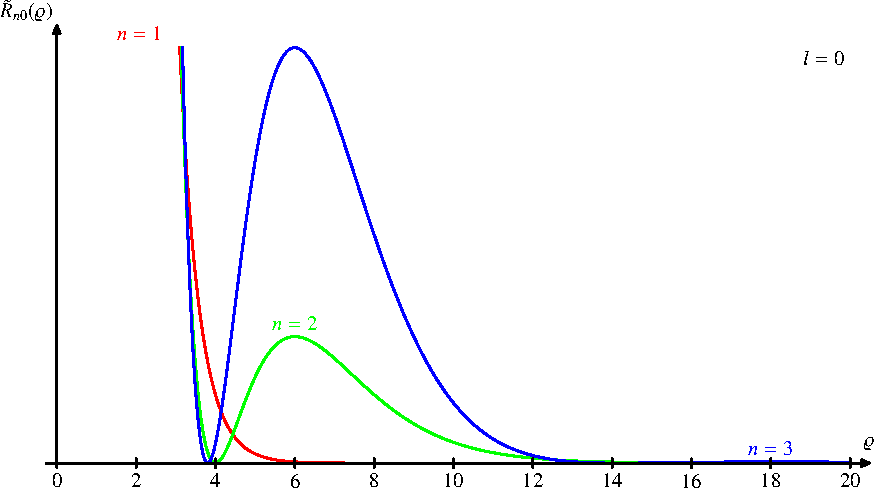
\includegraphics[width=\hsize]{graphics/radial-1.pdf}
\caption{Radiusabh"angigkeit der Wellenfunktionen in einem Wasserstoff-Atom
f"ur $l=0$.
\label{skript:radialgraphs-l0}}
\end{figure}

\begin{figure}
\centering
\includegraphics[width=\hsize]{graphics/radial-2.pdf}
\caption{Radiusabh"angigkeit der Wellenfunktionen in einem Wasserstoff-Atom
f"ur den Fall $l=n-1$,
Maximalwert auf $1$ normiert.
\label{skript:radialgraphs-maxl}}
\end{figure}

\subsection{p-Orbitale}
\index{p-Orbital}
Die p-Orbitale geh"oren zu $l=1$, somit gibt es drei Eigenfunktionen
entsprechenden den m"oglichen Werten $m=-1$, $m=0$ und $m=1$.
F"ur den Fall $m=0$ haben wir fr"uher gezeigt, dass
\[
P_1(z)=\frac{d}{dz}(z^2-1)=2z.
\]
Die Wellenfunktion h"angt aber nicht von $m$ ab.
Die Wahrscheinlichkeit, das Elektron in der N"ahe der $x$-$y$-Ebene
zu finden, ist also sehr klein.
Dieses Orbital wird auch p$\mathstrut_z$ genannt.

F"ur $m=\pm$ ist die $z$-Abh"angigkeit
\[
P_1^1(z)=2\sqrt{1-z^2} = 2\sin\vartheta,
\]
insbesondere ist f"ur diese Wellenfunktionen die Wahrscheinlichkeit 
am gr"ossten, das Elektron in der N"ahe der $x$-$y$-Ebene zu finden.
Die $\varphi$-Abh"angigkeit ist $e^{im\varphi}$, aber dies ist
nur ein Phasenfaktor.
Die Linearkombinationen
\[
e^{im\varphi}+e^{-im\varphi}=2\cos\varphi=2x
\qquad\text{und}\qquad
e^{im\varphi}-e^{-im\varphi}=2i\sin\varphi=2iy
\]
sind gleichwertige Wellenfunktionen.
Im ersten Fall h"alt sich das Elektron bevorzugt entlang der $x$-Achse
auf w"ahrend die Wahrscheinlichkeit f"ur $x$ klein also in der N"ahe der
$y$-$z$-Ebene sehr klein ist.
Im zweiten Fall meidet das Elektron die $y$-$z$-Ebene.
Diese Orbitale heissen auch $\text{p}_x$ und $\text{p}_y$
(Abbildung~\ref{skript:porbitale}).

\subsection{H"ohere Energie}
F"ur gr"ossere Werte der Quantenzahl $n$ sind auch gr"ossere Werte
von $l$ m"oglich.
F"ur $l=0$ befindet sich das Elektron zwar immer noch bevorzugt in 
Kernn"ahe, aber es sind zus"atzliche ``Schalen'' in gr"osserem Abstand
auszumachen (Abbildung~\ref{skript:radialgraphs-l0}).
F"ur $l=n-1$, dem gr"ossten m"oglichen Wert von $l$,
befindet sich das Elektron
bevorzugt in einer weit vom Atomkern entfernten Schale, wie die
Abbildung~\ref{skript:radialgraphs-maxl} zeigt.
Die Schalenstruktur entsteht also nicht ausschliesslich durch den 
Drehimpuls, sondern ist ein davon unabh"angiges ein Quantenph"anomen.
Man kann sich die Schale als eine radiale stehende Welle in dem
kugelsymmetrischen Potentialtopf des Atomkernes vorstellen.

\begin{figure}
\centering
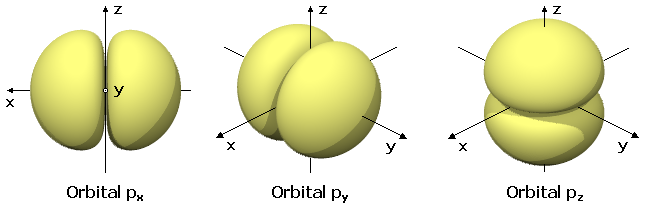
\includegraphics[width=\hsize]{images/orbital.png}
\caption{p-Orbitale dargestellt als Niveau-Fl"ache der Wellenfunktion
(Bildquelle: Wikipedia)
\label{skript:porbitale}}
\end{figure}

\begin{figure}
\centering
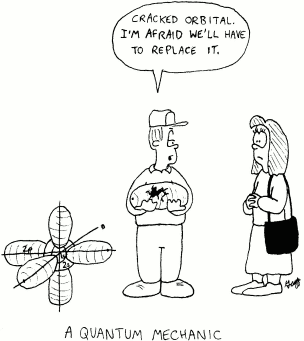
\includegraphics[width=0.4\hsize]{images/crackedorbital.png}
\caption{Berufsbild des Quantenmechanikers: Kenntnisse der Orbitale
sind unerl"asslich\label{skript:crackedorbital}}
\end{figure}
